\documentclass[border=2pt]{standalone}
\usepackage{pgfplots}
\pgfplotsset{compat=1.18}
\begin{document}
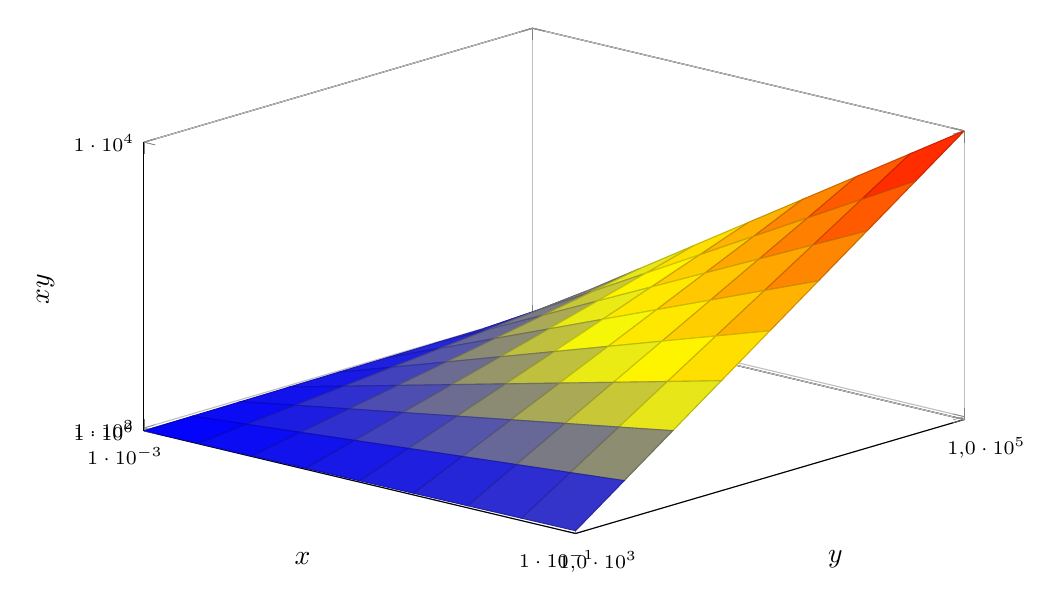
\begin{tikzpicture}
  \begin{axis}[
    width=12cm,
    height=8cm,
    view={42}{28},
    domain=0.001:0.1,
    y domain=1000:100000,
    samples=9,
    xmin=0.001,
    xmax=0.1,
    ymin=1000,
    ymax=100000,
    zmin=1,
    zmax=10000,
    xtick={0.001,0.1},
    ytick={1000,100000},
    ztick={1,100,10000},
    scaled ticks=false,
    tick label style={font=\scriptsize},
    xticklabel={$\pgfmathprintnumber[sci,precision=1]{\tick}$},
    yticklabel={$\pgfmathprintnumber[sci,sci zerofill,precision=1,use comma]{\tick}$},
    zticklabel={$\pgfmathprintnumber[sci,sci precision=2]{\tick}$},
    grid=major,
    xlabel={$x$},
    ylabel={$y$},
    zlabel={$xy$}
  ]
    \addplot3[surf] {x*y};
  \end{axis}
\end{tikzpicture}
\end{document}
